%%%%%%%%%%%%%%%%%%%%%%%%%%%%%%%%%%%%%%%%%%%%%%%%%%%%%%%%%%%%%%%%%%
%%%%%%%% ICML 2016 EXAMPLE LATEX SUBMISSION FILE %%%%%%%%%%%%%%%%%
%%%%%%%%%%%%%%%%%%%%%%%%%%%%%%%%%%%%%%%%%%%%%%%%%%%%%%%%%%%%%%%%%%

% Use the following line _only_ if you're still using LaTeX 2.09.
%\documentstyle[icml2016,epsf,natbib]{article}
% If you rely on Latex2e packages, like most moden people use this:
\documentclass{article}
\usepackage{amsmath}
% use Times
\usepackage{times}
% For figures
\usepackage{graphicx} % more modern
%\usepackage{epsfig} % less modern
\usepackage{subfigure} 

% For citations
\usepackage{natbib}

% For algorithms
\usepackage{algorithm}
\usepackage{algorithmic}

% As of 2011, we use the hyperref package to produce hyperlinks in the
% resulting PDF.  If this breaks your system, please commend out the
% following usepackage line and replace \usepackage{icml2016} with
% \usepackage[nohyperref]{icml2016} above.
\usepackage{hyperref}

% Packages hyperref and algorithmic misbehave sometimes.  We can fix
% this with the following command.
\newcommand{\theHalgorithm}{\arabic{algorithm}}
%\newcommand{\ICML@appearing}{}
% Employ the following version of the ``usepackage'' statement for
% submitting the draft version of the paper for review.  This will set
% the note in the first column to ``Under review.  Do not distribute.''
%\usepackage[accepted]{icml2016} 

% Employ this version of the ``usepackage'' statement after the paper has
% been accepted, when creating the final version.  This will set the
% note in the first column to ``Proceedings of the...''
\usepackage[accepted]{icml2016}


% The \icmltitle you define below is probably too long as a header.
% Therefore, a short form for the running title is supplied here:
\icmltitlerunning{Predictive Model for Time-Series Data with Bayesian Non-parametrics}

\begin{document} 

\twocolumn[
\icmltitle{Predictive Model for Time-Series Data with Bayesian Non-parametrics}

\vspace{-.15in}

% It is OKAY to include author information, even for blind
% submissions: the style file will automatically remove it for you
% unless you've provided the [accepted] option to the icml2016
% package.
\icmlauthor{Chawannut Prommin, cp626}{cp626@cornell.edu}
%\icmladdress{cp626}
\vspace{.05in}
\icmlauthor{Serena Li, sl2327}{sl2327@cornell.edu}
%\icmladdress{sl2327}
\vspace{.05in}
\icmlauthor{Yutao Han, yh675}{yh675@cornell.edu}
%\icmladdress{yh675}
\vspace{.05in}

% You may provide any keywords that you 
% find helpful for describing your paper; these are used to populate 
% the "keywords" metadata in the PDF but will not be shown in the document
\icmlkeywords{boring formatting information, machine learning, ICML}

\vskip 0.3in
]

\begin{abstract} 
We propose a novel model for time-series data using a Bayesian non-parametric framework. Training data is clustered into data patterns using the Indian Buffet Process, which is a flexible non-parametric model that allows each individual data point to be potentially assigned to multiple clusters. We also propose a framework to improve accuracy of online inference and extrapolation of the time-series data. We consider the scalability of the model during online inference due to evaluation of the clusters rather than the entire dataset, and scalability of the model during training by using approximate methods to learn the parameters of the non-parametric model.
\end{abstract} 
\vspace{-.25in}

\section{Introduction}

Time-series data in several domains is highly volatile and difficult to model (for example, stock prices fluctuate wildly and are difficult to model accurately) due to their often non-stationary nature. Essentially, different locations in input space produce outputs described with variable functions. The distinct locations where the functions that map inputs to outputs change are traditionally called change points. While difficult to model, there is significant motivation to learn time-series data for applications such as creating generative models of the stock market for financial gain or understanding seismic patterns to prevent catastrophe. 

A predictive model that identifies latent features within the data can be a powerful tool for understanding the time-series. It is intuitive to model the non stationarity of time-series data by using clustering methods to segment the time-series data into different patterns that correspond to the varying functions (with respect to input space) that model the outputs. Non-parametric models are good candidates to model time-series data because of they allow the complexity of the model to grow as more data is observed, which is central to modeling the non-stationarity of the data. Furthermore, non-parametric models do not have the limitations of physics-based models that make assumptions about the data such as optimizing trajectory distance, which can constrain the model and produce unrealistic results. The class of non-parametric models called Kernel Learning is ideal for modeling time-series data. Kernel learning uses kernel functions to learn the covariance, which roughly gives the expected difference in outputs given the inputs, of the data in function space allows for the flexibility of a non-parametric model, while also capturing uncertainty in a probabilistic manner. 

Given a model of time-series data, the ability for online inference is desired. As more data is observed online, the model should be able to update its parameters, cluster new data with existing patterns, and identify new patterns. The scalability of the model is a key point of concern as online learning needs to be done in real-time for maximum benefit. In addition to increasing the complexity of the model with online data, extrapolation of future data is desired. A Bayesian approach to online inference and extrapolation is appropriate in order to take advantage of the inductive biases in the model.

\section{Related Work} 
 
Previous work has modeled time-series data using purely non-parametric models \cite{FastNonP} and a combination of parametric and non-parametric models \cite{StructDiscNonPara}. Parametric models generally require less data to learn, but do not have the inherent flexibility of non-parametric models. Parametric models may be too heavily constrained to allow increases in model complexity given new observed data. Data-driven approaches have modeled time-series data with Gaussian Processes (GP) and Dirichlet Process Gaussian Process (DPGP) \cite{DPGPwithConstraints}. These approaches have had success in clustering multiple trajectories of time-series data, but do not identify clusters of points belonging to a pattern, which represent a variable functions mapping inputs to outputs of a single time-series trajectory. Identification of latent patterns or features would potentially allow for higher accuracy during online inference by allowing for interpretation of latent features describing the nature of the non-stationarity in the time-series. Other popular approaches to modeling time-series data find change points, which correspond to boundaries between variable functions, with a run-length variable and models the variable functions between change points accordingly \cite{GPChangePointModels}. A drawback of this type of approach is that the prior over the distribution of change points is not appropriate for modeling real data and a more statistically rigorous approach is desired. Approaches that find change points can be rather manual and we would prefer to automatically discover variations in underlying functions describing the data.

The Indian Buffet Process (IBP) is a non-parametric model that can discover latent features in data and is most commonly used in clustering problems (for example, clustering images based on latent features). The IBP allows for each individual data point to be assigned multiple latent features which allows for more flexibility than traditional clustering approaches. There has been application of the IBP to clustering multiple time-series trajectories and learn compositions of GP kernels describing the clusters \cite{IBPGP}. However, this approach uses predefined kernels (such as the RBF or periodic kernels) and the compositions of kernels are limited to summation. A general kernel function that can learn complex patterns and provide interpretable results is desired. [Ref] developed a powerful Spectral Mixture (SM) kernel for GP regression which can theoretically can model any stationary kernel. The SM kernel has shown promising results in learning complex patterns and in performing accurate extrapolation. In addition, the SM kernel allows for direct analysis of the spectral density of the kernel which facilitates interpretability of the kernel.

The non-parametric nature of the IBP means it can quickly become intractable given the complexity of the data. [Ref] performs fast inference with the IBP by using a mean varitional method. Modeling with GPs can also cause scalability problems due to the complexity of inverting the kernel matrix; the community has developed approximation methods that exploit kernel matrix structure for fast inference \cite{KISS-GP}.

\section{Methodology}

\subsection{Contribution}
Figure \ref{AlgFlow} shows the algorithmic flow of our model. We propose an IBP clustering process to cluster time-series data. Our model then uses GP regression with a SM kernel to learn the correlations on data for each cluster. Finally, our method performs online inference by using a chi-squared goodness of fit test for clustering new data and updating model parameters.

\begin{figure}[ht]
\vskip 0.2in
\begin{center}
\centerline{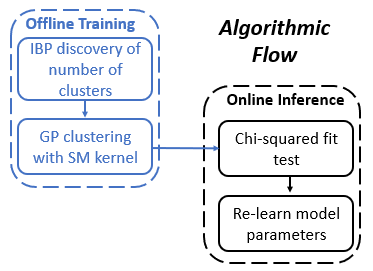
\includegraphics[width=\columnwidth]{AlgFlow}}
\caption{Algorithmic flow of the proposed time-series model. In offline training (light blue) the data is clustered into patterns with the IBP process and then GP regression is preformed over each cluster with the SM kernel. In online inference (black) the model performs chi-squared goodness of fit tests to cluster new data and then re-learns SM kernel hyperparameters for the cluster.}
\label{AlgFlow}
\end{center}
\vskip -0.2in
\end{figure} 

\subsection{Indian Buffet Process (IBP) Clustering}
%Finding the hidden structure of time-series data using latent feature modeling is the first step in our model. In short, given a data set $X$ with $n$ objects and $d$ dimensions, latent feature modeling aims to decompose $X$ to a binary feature matrix $Z$ with $n$ rows and $k$ columns, a weight matrix $A$ with $k$ rows and $d$ columns, and white noise $\epsilon$. One interpretation of each row of matrix $Z$ is whether each object possesses latent feature $k$ or not. 
%
%$$
%X^{nxd}=Z^{nxk}A^{kxd}+\epsilon_{nxd}
%\eqno{(1)}
%$$
%
%In order to do inference, we first need a prior over the binary matrix $Z$. The IBP is a non-parametric model which gives a prior over binary matrix where $z_{ij} = 1$ if object $i$ possess latent feature $k$ and $z_{ij} =  0$ otherwise. [Ref] derives the closed form of the IBP process [eq]?. There are two equivalent ways to generate samples from the IBP process. 
%
%Traditional clustering method assign one data point to one cluster while Indian Buffet Process does not has such constraint.Also,another major drawback of traditional clustering method is that the number of cluster (K) need to be predefined.However, in nonparametric model, the number of cluster is not fixed and can grow overtime as we have more data.The figure show how can we interpret the process of assigning data point to cluster in term of binary matrix.The figure on the left represent traditional clustering method where each row can only belong to one column while the figure on the right show that one figure can belong to multiple clusters.


\subsection{Spectral Mixture (SM) Kernel Learning}

GP regression is used to learn each cluster from the IBP process. A GP learns correlations between the output functions of inputs for given data. The outputs are not assumed to take any functional form and are a normal random vector. The kernel function of the GP describes the covariance between the outputs which roughly is the divergence of the outputs given their inputs. The kernel function has hyperparameters which determine properties of the functions drawn from the GP such as length scale or frequency. We assume white measurement noise. The distribution of output functions is given below.

$$
\begin{bmatrix} 
y(x) \\
y(x_{*}) 
\end{bmatrix}
=
\begin{bmatrix} 
K+\sigma_{n}^{2}I & K_{*} \\
K_{*} & K_{**} 
\end{bmatrix}
\eqno(1)
$$

Where $x$ is the training input, $y(x)$ is the training output, $x_{*}$ is the input where we would like to predict the output $y(x_{*})$ with GP regression, $\sigma_{n}^{2}$ is the measurement noise hyperparameter, $K$ is the kernel function and describes the covariance points between the set of points $\{x,x\}$, $K_{*}$ is the covariance between $\{x_{*},x\}$, and $K_{**}$ is the covariance between $\{x_{*},x_{*}\}$. From now on $y(x)$ will be denoted as $y$, and $y(x_{*})$ will be denoted as $y^{*}$. With some linear algebra the marginal distribution of $y^{*}$ is derived as:

$$
y^*\sim \mathcal{N}(K_{*}^{T}K^{-1}y,K_{**}-K_{*}^{T}K^{-1}K_{*})  \eqno{(2)}
$$


A stationary kernel function is one that only depends on the norm between the inputs. Generally, kernel functions are hand-crafted to fit specific problems and require significant human time to fine tune. An alternative kernel modeling method that automatically discovers an appropriate kernel function is desired. [ref] The spectral density can be used to model the stationary kernel and by taking a mixture of gaussians in the spectral representation, any stationary kernel can be modeled. The inverse Fourier transform of the spectral representation is the SM kernel. The SM kernel function is defined as follows:

%$$
%\phi(s;\mu,\sigma^{2})=\frac{1}{\sqrt{2\pi\sigma^{2}}}\textrm{exp}\{-\frac{1}{2\sigma^{2}}(s-\mu)^{2}\}
%\eqno(1)
%$$
$$
S(s)=\frac{1}{2}[\phi(s)+\phi(-s)]
\eqno(1)
$$
%$$
%K(\tau)=\textrm{exp}\{-2\pi^{2}\tau^{2}\sigma^{2}\}\textrm{cos}(2\pi\tau\mu)
%\eqno(1)
%$$
$$
K(\tau)=\sum_{q=1}^{Q}w_{q}\prod_{p=1}^{P}\textrm{exp}\{-2\pi^{2}\tau_{p}^{2}v_{q}^{(p)}\}\textrm{cos}(2\pi\tau_{p}\mu_{q}^{(p)})
\eqno{(5)}
$$
Where $\phi(s)$ is a mixture of $Q$ Gaussians with the $q^{th}$ component having mean vector $\mu_{q}=\{\mu_{q}^{(1)},...\mu_{q}^{(P)}\}$ and diagonal covariance matrix with diagonal components $v_{q}=\{v_{q}^{(1)},...v_{q}^{(P)}\}$, $S(s)$ is the spectral density of the kernel function $K$, and $\tau_{p}$ is the $p^{th}$ component of the $P$ dimensional vector of difference in inputs [ref]. While the the time-series data is non-stationary in nature, the clusters found by the IBP are stationary and can be appropriately modeled by the SM kernel. As $Q$ goes to infinity, any stationary kernel can be modeled by the SM kernel exactly. This is not feasible in practice, so a value of $Q$ that learns the data patterns reasonably well is empirically determined.

We can learn the hyperparameters $\theta=\{w,\mu,v,\sigma_{n}\}$ of the kernel by maximizing the marginal likelihood of the data

$$
\textrm{log}\ p(y|\theta) \propto -y^{T}M^{-1}y -\textrm{log}\ |M|
\eqno(1)
$$
$$
M=K+\sigma_{n}^{2}I
\eqno(1)
$$

The gradient of the log likelihood is used for optimization, and is written as
$$
\frac{\partial}{\partial\theta}\textrm{log}\ p(y|\theta)=\frac{1}{2}y^TM^{-1}\frac{\partial M}{\partial\theta}M^{-1}y
$$
$$
-\frac{1}{2}\textrm{tr}(M^{-1}\frac{\partial M}{\partial\theta})
\eqno{(4)}
$$

The hyperparameters of the kernel function essentially determine the inferred distribution over functions at $x_{*}$. It is naturally appropriate to continuously update $\theta$ as more data is learned for the GP to achieve the best possible fit.

\subsection{Online Inference}

In online inference, our model clusters new data observed online with existing patterns or generates new clusters for the new data. The model updates clusters kernel hyperparameters as new data is found, and is more scalable because hyperparameters are optimized over clusters rather than the entire dataset.

When new data is observed online, the model first performs chi-squared goodness of fit tests on the observed data and each cluster learned during the model training. The model subsequently groups the online data into the cluster with the best "fit". If the data does not fit any existing clusters with a predefined level of confidence then a new cluster is generated. The test statistic for the chi-squared test is defined below:

$$
	t_{\chi^{2}}^{n_{y}}=(y(x_{*})-y)^{T}P^{-1}(y(x_{*})-y)
	\eqno{(1)}
$$
$$	
	P=K_{**}+\sigma_{n}^{2}I
	\eqno{(2)}
	$$

Where $y$ is the observed output at the new input $x_{*}$ online, $y(x_{*})$ is the expected output at $x_{*}$ given the SM kernel, $K_{**}$ is the covariance at $x_{*}$ given the SM kernel, $\sigma_{n}^{2}$ is the noise hyperparameter of the SM kernel, and ${n_{y}}$ is the dimension of $y$. The test statistic $t_{\chi^{2}}^{n_{y}}$ is chi-squared distributed with ${n_{y}}$ degrees of freedom. If we are more than $90\%$ confident that $y$ was generated by the learned distribution over a cluster from the training data with the SM kernel, then the new data is assigned to that cluster. If the new data is more than $90\%$ confident to belong to multiple clusters, then we assign the new data to the cluster with the highest confidence. If the new data cannot be assigned to any cluster with $90\%$ confidence then it is assigned to a new cluster. 

After the new points are assigned to a cluster, the hyperparameters of the SM kernel over the cluster are relearned through marginal likelihood. Rather than re-optimizing hyperparameters over the entire dataset, our model only optimizes over a subset of the data defined by the cluster, which makes the model scalable. However, huge datasets will eventually bottleneck when the clusters grow extremely large so approximation methods must be used. We use point inducing methods for fast inference of the GP. We assign new data to clusters after a predetermined number $N_{new}$ of new data points are observed. If $N_{new}$ is too small, then the chi-squared test may not be representative and it will be computationally expensive to re-learn hyperparameters for each new set of clustered $N_{new}$ points. However, if $N_{new}$ is too large then the resolution may not be small enough to correctly cluster the new points. $N_{new}$ is empirically found in the model.

The SM kernel also allows the model to perform short-term extrapolation of data by assuming the extrapolated points will belong the most recently assigned cluster. Naturally, this method is only accurate for short term extrapolation due to the non-stationary nature of time-series data.

\section{Experimental Results}

\section{Discussion}

\bibliography{example_paper}
\bibliographystyle{icml2016}

\end{document} 


% This document was modified from the file originally made available by
% Pat Langley and Andrea Danyluk for ICML-2K. This version was
% created by Lise Getoor and Tobias Scheffer, it was slightly modified  
% from the 2010 version by Thorsten Joachims & Johannes Fuernkranz, 
% slightly modified from the 2009 version by Kiri Wagstaff and 
% Sam Roweis's 2008 version, which is slightly modified from 
% Prasad Tadepalli's 2007 version which is a lightly 
% changed version of the previous year's version by Andrew Moore, 
% which was in turn edited from those of Kristian Kersting and 
% Codrina Lauth. Alex Smola contributed to the algorithmic style files.  
